\documentclass[problems]{esg8012pset} 
  \usepackage{amsmath}
  \usepackage{amssymb}
  \usepackage{enumerate}
  \usepackage{graphicx}
  \providecommand{\uvec}[1]{{\hat{\bf{#1}}}}
  \usepackage{pgf,tikz}
  \usetikzlibrary{arrows}
  \makeatletter
  \newcommand{\interitemtext}[1]{%
    \begin{list}{}
     {\itemindent=0mm\labelsep=0mm
     \labelwidth=0mm\leftmargin=0mm
     \addtolength{\leftmargin}{-\@totalleftmargin}}
      \item #1
    \end{list}
  }
  \makeatother
  \renewcommand{\d}{\,d}
  \providecommand{\norm}[1]{\lVert#1\rVert}
\classname{Physics 8.012} 
\semester{Fall 2010} 
\problemsetnumber{3} 
\date{September 24} 
\duedate{Friday, October 1} 
\readingassignment{Kleppner and Kolenkow, \emph {An Introduction to Mechanics}, Chapter Two} 
\begin{document}
\section*{Problem 1: K\&K 2.24}
  A device called a capstan is used aboard ships in order to control a rope which is under great tension. The rope is wrapped around a fixed drum, usually for several turns (the drawing shows about three fourths turn). The load on the rope pulls it with a force $T_A$, and the sailor holds it with a much smaller force $T_B$.  Can you show that $T_B = T_Ae^{-\mu_s\theta}$, where $\mu_s$ is the coefficient of static friction and $\theta$ is the total angle subtended by the rope on the drum?
  \begin{center}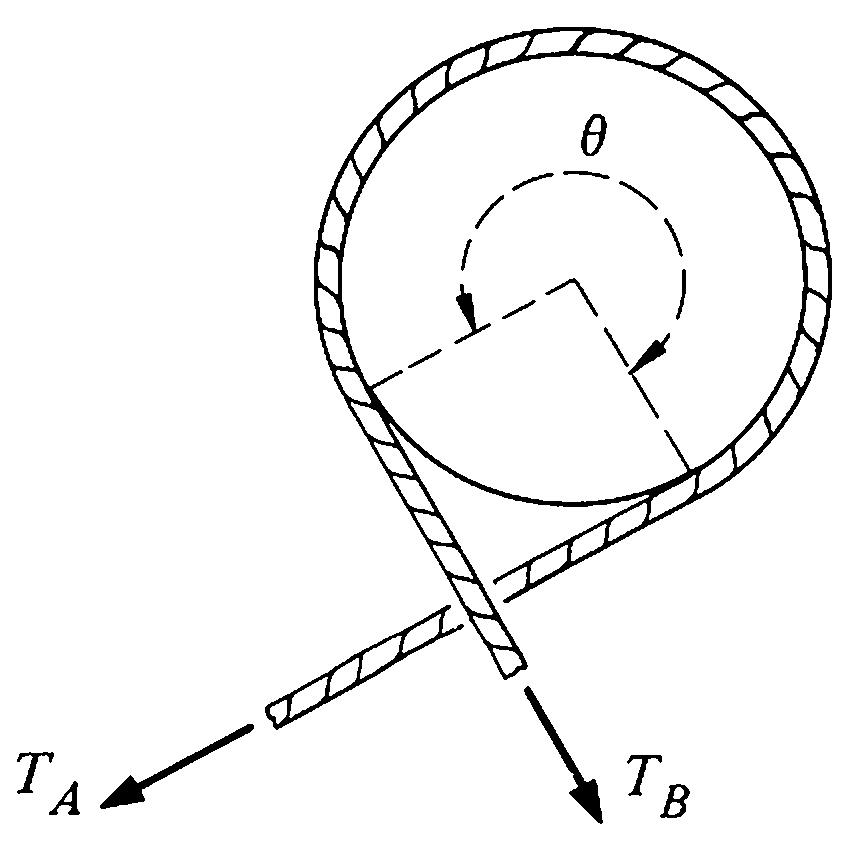
\includegraphics[width=0.35\textwidth]{ps03_1}\end{center}
\section*{Problem 2: The Gravitational Field of a Spherical Shell of Matter}
  Consider a spherical shell of radius $R$ of mass $m_s$, that is uniformly distributed over the shell with mass per unit area $\sigma = \frac{m_s}{4\pi R^2}$.  Show that
  \begin{enumerate}[1)]
    \item The gravitational force on a mass m placed outside a spherical shell of matter of uniform surface mass density $\sigma$ is the same force that would arise if all the mass of the shell were placed at the center of the sphere.
    \item The gravitational force on a mass m placed inside a spherical shell of matter is zero.
  \interitemtext{$$\vec{\bf{F}}_{m,s}(r) = \begin{cases} -G\frac{mm_s}{r^2}\hat{\bf r} & r > R \\ \vec{\bf{0}} & r < R\end{cases}$$
  where $\hat{\bf{r}}$ is the unit vector located at the position of mass $m$ and pointing radially away from the center of the shell.

  Now consider a solid uniform sphere of mass $m_T$ and radius $R$.}
    \item Show that the gravitational force on a body of mass $m$, uniform mass density $\rho = \frac{m_r}{\frac{4}{3}\pi R^3}$, located a distance $r<R$, is due solely to the mass lying at a distance $r'\leq r$, measured from the center of the sphere, and is given by $\vec{\bf{F}}_{m,s}(r)=-\frac{4\pi}{3}Gm\rho r\hat{\bf{r}}$, $r<R$.
  \end{enumerate}
\section*{Problem 3: K\&K 2.26 (Simple Harmonic Motion: Tunnel through the earth)}
  Suppose a tunnel is drilled through the earth passing through the center. The earth has radius $R$, total mass $m$ and uniform mass density $\rho = \frac{m}{\frac{4}{3}\pi R^3}$.  If an object is released at one end of the tunnel, how long will it take the object to return to the starting point?

  You may assume that the earth is a uniformly dense sphere, and you must neglect all friction and any effects due to the earth's rotation.
  \begin{center}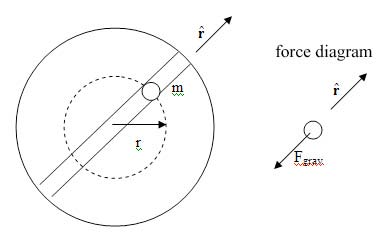
\includegraphics[width=0.35\textwidth]{ps03_2}\end{center}
\section*{Problem 4: K\&K 2.28 (Circular motion: banked turn)}
  A car of mass $m$ is going around a circular turn of radius $R$ which is banked at an angle $\theta$ with respect to the ground. Assume there is a coefficient of static friction $\mu_s$ between the wheels and the road. Let $g$ be the magnitude of the acceleration due to gravity. You may neglect kinetic friction. In each part below show your force diagrams.
  \begin{enumerate}[a)]
    \item Derive an expression for the minimum velocity necessary to keep the car moving in a circle without slipping down the embanked turn. Express your answer in terms of the given quantities.
    \item Derive an expression for the maximum velocity necessary to keep the car moving in a circle without slipping up the embanked turn. Express your answer in terms of the given quantities.
    \item Derive an expression for the velocity necessary to keep the car moving in a circle without slipping up or down the embanked turn such that the static friction force vanishes. Express your answer in terms of the given quantities.
  \end{enumerate}
  \begin{center}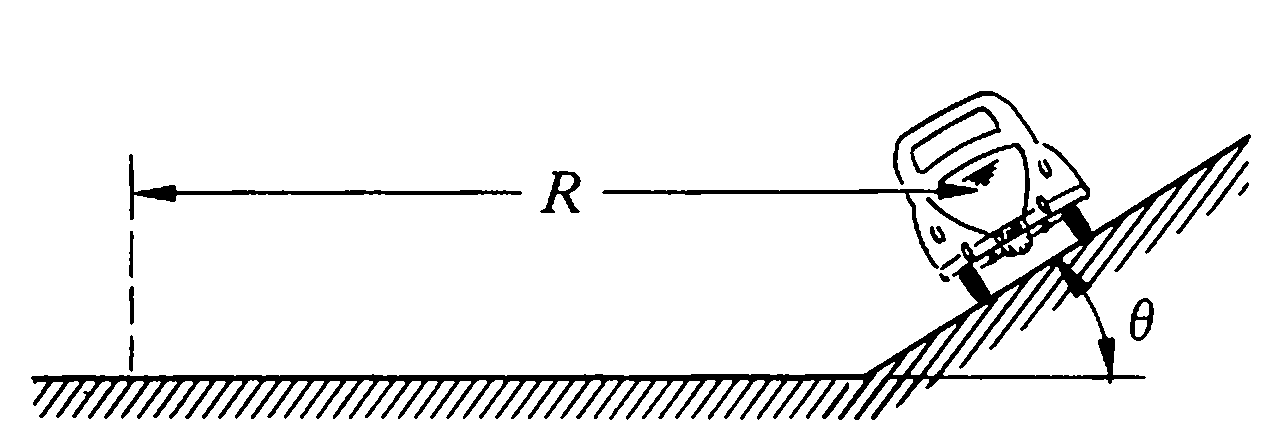
\includegraphics[width=0.35\textwidth]{ps03_3}\end{center}
\section*{Problem 5: K\&K 2.31}
  Find the frequency of oscillation of a block of mass $m$ suspending by two springs having spring constants $k_1$ and $k_2$,
  \begin{center}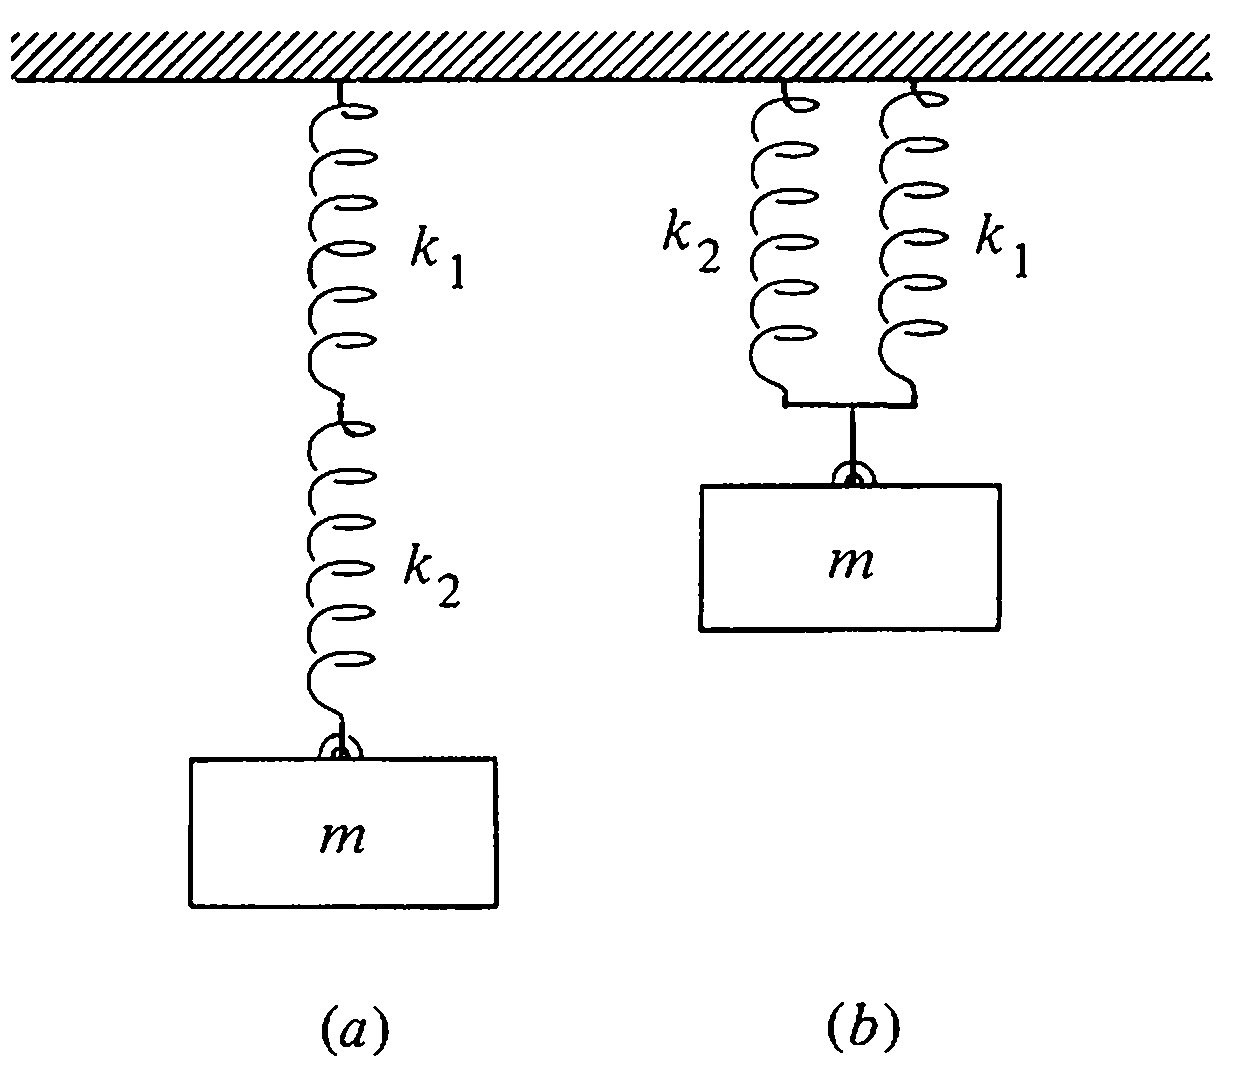
\includegraphics[width=0.35\textwidth]{ps03_4}\end{center}
  \begin{enumerate}[a)]
    \item when they are each attached to the wall and the block (in parallel);
    \item when spring 1 is attached to the wall and one end of spring 2 , and the other end of spring 2 is attached to the block (in series).
  \end{enumerate}
\section*{Problem 6: K\&K 2.34}
  A body of mass $m$ whirls around on a string which passes through a fixed ring located at the center of the circular motion. The string is held by a person who pulls the string downward with a constant velocity of magnitude $V$ so that the radial distance to the body decreases. Initially the body is a distance $r_0$ from the center and is revolving
with angular velocity $\omega_0$. You may neglect the effect of gravity.
  \begin{enumerate}[a)]
    \item Draw a free body force diagram for body. Identify which coordinates you will choose and draw the unit vectors associated with your coordinate system on your free body diagram.
    \item Using Newton's second laws, derive a differential equation for the angular velocity $\omega$.
    \item Solve the differential equation for $\omega$ by integration techniques and using the initial conditions, find an expression for the angular velocity as a function of time, $\omega(t)$.
    \item Find the force needed to pull the string.
    \item Compute the quantity, $\vec{\bf{L}} = \vec{\bf{r}}\times m\vec{\bf{v}}$, (this is called the \emph{angular momentum}). Does this quantity change in time as the body moves in a spirally inward motion?
  \end{enumerate}
\section*{Problem 7: K\&K 2.36}
  A particle of mass $m$ moving along a straight line is acted on by a velocity dependent retarding force (one always directed against the motion) of magnitude $F = be^{\alpha v}$, where $b$ and $\alpha$ are constants and $v$ is the magnitude of the velocity (speed). At $t = 0$, the particle is moving with speed $v_0$. Find the velocity as a function of time $t$, $v(t)$.
\section*{Problem 8: K\&K 2.37}
  The Eureka Hovercraft Corporation wanted to hold hovercraft races as an advertising stunt. The hovercraft supports itself by blowing air downward, and has a big fixed propeller on the top deck for forward propulsion. Unfortunately it has no steering equipment, so that pilots found that making high speed turns was very difficult. The company decided to overcome this problem by designing a bowl shaped track in which the hovercraft, once up to speed, would coast along in a circular path with no need to steer. They hired an engineer to design and build the track, and when he finished, he hastily left the country. When the company held their first race, they found to their dismay that the craft took exactly the same time $T$ to circle the track, no matter what speed.
  \begin{enumerate}[a)]
    \item Explain how it is possible that the time is independent of the speed.
    \item Find the equation for the height of the cross section of the bowl in terms of the period to complete one revolution $T$.
  \end{enumerate}
\end{document}
